% Circulant Ramsey colourings (generated by figs_c1ch08.py).
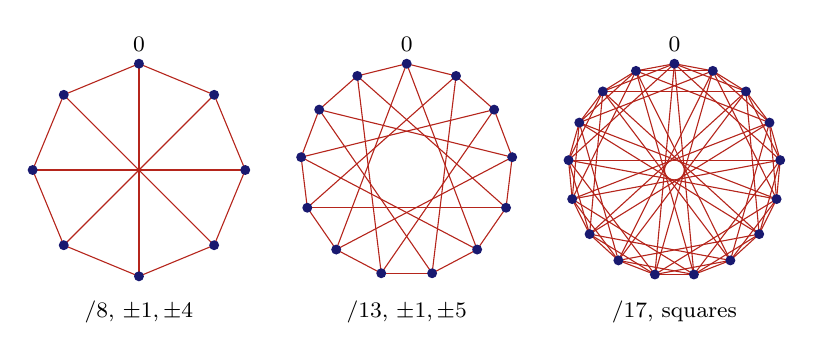
\begin{tikzpicture}[x=1cm,y=1cm,v/.style={circle,fill=MidnightBlue,inner sep=1.6pt},e/.style={MidnightBlue!70},l/.style={font=\footnotesize}]
\draw[BrickRed,thin] (0.000,1.350) -- (0.955,0.955);
\draw[BrickRed,thin] (0.000,1.350) -- (0.000,-1.350);
\draw[BrickRed,thin] (0.000,1.350) -- (-0.955,0.955);
\draw[BrickRed,thin] (0.955,0.955) -- (1.350,0.000);
\draw[BrickRed,thin] (0.955,0.955) -- (-0.955,-0.955);
\draw[BrickRed,thin] (1.350,0.000) -- (0.955,-0.955);
\draw[BrickRed,thin] (1.350,0.000) -- (-1.350,-0.000);
\draw[BrickRed,thin] (0.955,-0.955) -- (0.000,-1.350);
\draw[BrickRed,thin] (0.955,-0.955) -- (-0.955,0.955);
\draw[BrickRed,thin] (0.000,-1.350) -- (-0.955,-0.955);
\draw[BrickRed,thin] (-0.955,-0.955) -- (-1.350,-0.000);
\draw[BrickRed,thin] (-1.350,-0.000) -- (-0.955,0.955);
\fill[MidnightBlue] (0.000,1.350) circle (1.8pt);
\node[l] at (0.000,1.600) {$0$};
\fill[MidnightBlue] (0.955,0.955) circle (1.8pt);
\fill[MidnightBlue] (1.350,0.000) circle (1.8pt);
\fill[MidnightBlue] (0.955,-0.955) circle (1.8pt);
\fill[MidnightBlue] (0.000,-1.350) circle (1.8pt);
\fill[MidnightBlue] (-0.955,-0.955) circle (1.8pt);
\fill[MidnightBlue] (-1.350,-0.000) circle (1.8pt);
\fill[MidnightBlue] (-0.955,0.955) circle (1.8pt);
\node[l] at (0,-1.8) {$\Z/8\Z$, $\pm1,\pm4$};
\draw[BrickRed,thin] (3.400,1.350) -- (4.027,1.195);
\draw[BrickRed,thin] (3.400,1.350) -- (4.295,-1.010);
\draw[BrickRed,thin] (3.400,1.350) -- (2.505,-1.010);
\draw[BrickRed,thin] (3.400,1.350) -- (2.773,1.195);
\draw[BrickRed,thin] (4.027,1.195) -- (4.511,0.767);
\draw[BrickRed,thin] (4.027,1.195) -- (3.723,-1.311);
\draw[BrickRed,thin] (4.027,1.195) -- (2.138,-0.479);
\draw[BrickRed,thin] (4.511,0.767) -- (4.740,0.163);
\draw[BrickRed,thin] (4.511,0.767) -- (3.077,-1.311);
\draw[BrickRed,thin] (4.511,0.767) -- (2.060,0.163);
\draw[BrickRed,thin] (4.740,0.163) -- (4.662,-0.479);
\draw[BrickRed,thin] (4.740,0.163) -- (2.505,-1.010);
\draw[BrickRed,thin] (4.740,0.163) -- (2.289,0.767);
\draw[BrickRed,thin] (4.662,-0.479) -- (4.295,-1.010);
\draw[BrickRed,thin] (4.662,-0.479) -- (2.138,-0.479);
\draw[BrickRed,thin] (4.662,-0.479) -- (2.773,1.195);
\draw[BrickRed,thin] (4.295,-1.010) -- (3.723,-1.311);
\draw[BrickRed,thin] (4.295,-1.010) -- (2.060,0.163);
\draw[BrickRed,thin] (3.723,-1.311) -- (3.077,-1.311);
\draw[BrickRed,thin] (3.723,-1.311) -- (2.289,0.767);
\draw[BrickRed,thin] (3.077,-1.311) -- (2.505,-1.010);
\draw[BrickRed,thin] (3.077,-1.311) -- (2.773,1.195);
\draw[BrickRed,thin] (2.505,-1.010) -- (2.138,-0.479);
\draw[BrickRed,thin] (2.138,-0.479) -- (2.060,0.163);
\draw[BrickRed,thin] (2.060,0.163) -- (2.289,0.767);
\draw[BrickRed,thin] (2.289,0.767) -- (2.773,1.195);
\fill[MidnightBlue] (3.400,1.350) circle (1.8pt);
\node[l] at (3.400,1.600) {$0$};
\fill[MidnightBlue] (4.027,1.195) circle (1.8pt);
\fill[MidnightBlue] (4.511,0.767) circle (1.8pt);
\fill[MidnightBlue] (4.740,0.163) circle (1.8pt);
\fill[MidnightBlue] (4.662,-0.479) circle (1.8pt);
\fill[MidnightBlue] (4.295,-1.010) circle (1.8pt);
\fill[MidnightBlue] (3.723,-1.311) circle (1.8pt);
\fill[MidnightBlue] (3.077,-1.311) circle (1.8pt);
\fill[MidnightBlue] (2.505,-1.010) circle (1.8pt);
\fill[MidnightBlue] (2.138,-0.479) circle (1.8pt);
\fill[MidnightBlue] (2.060,0.163) circle (1.8pt);
\fill[MidnightBlue] (2.289,0.767) circle (1.8pt);
\fill[MidnightBlue] (2.773,1.195) circle (1.8pt);
\node[l] at (3.4,-1.8) {$\Z/13\Z$, $\pm1,\pm5$};
\draw[BrickRed,thin] (6.800,1.350) -- (7.288,1.259);
\draw[BrickRed,thin] (6.800,1.350) -- (7.709,0.998);
\draw[BrickRed,thin] (6.800,1.350) -- (8.144,0.125);
\draw[BrickRed,thin] (6.800,1.350) -- (7.048,-1.327);
\draw[BrickRed,thin] (6.800,1.350) -- (6.552,-1.327);
\draw[BrickRed,thin] (6.800,1.350) -- (5.456,0.125);
\draw[BrickRed,thin] (6.800,1.350) -- (5.891,0.998);
\draw[BrickRed,thin] (6.800,1.350) -- (6.312,1.259);
\draw[BrickRed,thin] (7.288,1.259) -- (7.709,0.998);
\draw[BrickRed,thin] (7.288,1.259) -- (8.008,0.602);
\draw[BrickRed,thin] (7.288,1.259) -- (8.098,-0.369);
\draw[BrickRed,thin] (7.288,1.259) -- (6.552,-1.327);
\draw[BrickRed,thin] (7.288,1.259) -- (6.089,-1.148);
\draw[BrickRed,thin] (7.288,1.259) -- (5.592,0.602);
\draw[BrickRed,thin] (7.288,1.259) -- (6.312,1.259);
\draw[BrickRed,thin] (7.709,0.998) -- (8.008,0.602);
\draw[BrickRed,thin] (7.709,0.998) -- (8.144,0.125);
\draw[BrickRed,thin] (7.709,0.998) -- (7.877,-0.814);
\draw[BrickRed,thin] (7.709,0.998) -- (6.089,-1.148);
\draw[BrickRed,thin] (7.709,0.998) -- (5.723,-0.814);
\draw[BrickRed,thin] (7.709,0.998) -- (5.891,0.998);
\draw[BrickRed,thin] (8.008,0.602) -- (8.144,0.125);
\draw[BrickRed,thin] (8.008,0.602) -- (8.098,-0.369);
\draw[BrickRed,thin] (8.008,0.602) -- (7.511,-1.148);
\draw[BrickRed,thin] (8.008,0.602) -- (5.723,-0.814);
\draw[BrickRed,thin] (8.008,0.602) -- (5.502,-0.369);
\draw[BrickRed,thin] (8.008,0.602) -- (6.312,1.259);
\draw[BrickRed,thin] (8.144,0.125) -- (8.098,-0.369);
\draw[BrickRed,thin] (8.144,0.125) -- (7.877,-0.814);
\draw[BrickRed,thin] (8.144,0.125) -- (7.048,-1.327);
\draw[BrickRed,thin] (8.144,0.125) -- (5.502,-0.369);
\draw[BrickRed,thin] (8.144,0.125) -- (5.456,0.125);
\draw[BrickRed,thin] (8.098,-0.369) -- (7.877,-0.814);
\draw[BrickRed,thin] (8.098,-0.369) -- (7.511,-1.148);
\draw[BrickRed,thin] (8.098,-0.369) -- (6.552,-1.327);
\draw[BrickRed,thin] (8.098,-0.369) -- (5.456,0.125);
\draw[BrickRed,thin] (8.098,-0.369) -- (5.592,0.602);
\draw[BrickRed,thin] (7.877,-0.814) -- (7.511,-1.148);
\draw[BrickRed,thin] (7.877,-0.814) -- (7.048,-1.327);
\draw[BrickRed,thin] (7.877,-0.814) -- (6.089,-1.148);
\draw[BrickRed,thin] (7.877,-0.814) -- (5.592,0.602);
\draw[BrickRed,thin] (7.877,-0.814) -- (5.891,0.998);
\draw[BrickRed,thin] (7.511,-1.148) -- (7.048,-1.327);
\draw[BrickRed,thin] (7.511,-1.148) -- (6.552,-1.327);
\draw[BrickRed,thin] (7.511,-1.148) -- (5.723,-0.814);
\draw[BrickRed,thin] (7.511,-1.148) -- (5.891,0.998);
\draw[BrickRed,thin] (7.511,-1.148) -- (6.312,1.259);
\draw[BrickRed,thin] (7.048,-1.327) -- (6.552,-1.327);
\draw[BrickRed,thin] (7.048,-1.327) -- (6.089,-1.148);
\draw[BrickRed,thin] (7.048,-1.327) -- (5.502,-0.369);
\draw[BrickRed,thin] (7.048,-1.327) -- (6.312,1.259);
\draw[BrickRed,thin] (6.552,-1.327) -- (6.089,-1.148);
\draw[BrickRed,thin] (6.552,-1.327) -- (5.723,-0.814);
\draw[BrickRed,thin] (6.552,-1.327) -- (5.456,0.125);
\draw[BrickRed,thin] (6.089,-1.148) -- (5.723,-0.814);
\draw[BrickRed,thin] (6.089,-1.148) -- (5.502,-0.369);
\draw[BrickRed,thin] (6.089,-1.148) -- (5.592,0.602);
\draw[BrickRed,thin] (5.723,-0.814) -- (5.502,-0.369);
\draw[BrickRed,thin] (5.723,-0.814) -- (5.456,0.125);
\draw[BrickRed,thin] (5.723,-0.814) -- (5.891,0.998);
\draw[BrickRed,thin] (5.502,-0.369) -- (5.456,0.125);
\draw[BrickRed,thin] (5.502,-0.369) -- (5.592,0.602);
\draw[BrickRed,thin] (5.502,-0.369) -- (6.312,1.259);
\draw[BrickRed,thin] (5.456,0.125) -- (5.592,0.602);
\draw[BrickRed,thin] (5.456,0.125) -- (5.891,0.998);
\draw[BrickRed,thin] (5.592,0.602) -- (5.891,0.998);
\draw[BrickRed,thin] (5.592,0.602) -- (6.312,1.259);
\draw[BrickRed,thin] (5.891,0.998) -- (6.312,1.259);
\fill[MidnightBlue] (6.800,1.350) circle (1.8pt);
\node[l] at (6.800,1.600) {$0$};
\fill[MidnightBlue] (7.288,1.259) circle (1.8pt);
\fill[MidnightBlue] (7.709,0.998) circle (1.8pt);
\fill[MidnightBlue] (8.008,0.602) circle (1.8pt);
\fill[MidnightBlue] (8.144,0.125) circle (1.8pt);
\fill[MidnightBlue] (8.098,-0.369) circle (1.8pt);
\fill[MidnightBlue] (7.877,-0.814) circle (1.8pt);
\fill[MidnightBlue] (7.511,-1.148) circle (1.8pt);
\fill[MidnightBlue] (7.048,-1.327) circle (1.8pt);
\fill[MidnightBlue] (6.552,-1.327) circle (1.8pt);
\fill[MidnightBlue] (6.089,-1.148) circle (1.8pt);
\fill[MidnightBlue] (5.723,-0.814) circle (1.8pt);
\fill[MidnightBlue] (5.502,-0.369) circle (1.8pt);
\fill[MidnightBlue] (5.456,0.125) circle (1.8pt);
\fill[MidnightBlue] (5.592,0.602) circle (1.8pt);
\fill[MidnightBlue] (5.891,0.998) circle (1.8pt);
\fill[MidnightBlue] (6.312,1.259) circle (1.8pt);
\node[l] at (6.8,-1.8) {$\Z/17\Z$, squares};
\end{tikzpicture}
